% Results section for Idea C: Quantization Impact on Structured Web Data Extraction
% Include with: % Results section for Idea C: Quantization Impact on Structured Web Data Extraction
% Include with: % Results section for Idea C: Quantization Impact on Structured Web Data Extraction
% Include with: % Results section for Idea C: Quantization Impact on Structured Web Data Extraction
% Include with: \input{sections/results}

\section{Results}
\label{sec:results}

We evaluate four small language models across multiple GGUF quantization levels on 100 web pages from the ScrapeGraphAI-100k dataset, measuring extraction quality (F1), JSON output validity, and inference latency.

\subsection{Experimental Setup}

We test four model families: Qwen2.5-3B-Instruct, Llama-3.2-3B-Instruct, Phi-3.5-mini-Instruct (3.8B), and Mistral-7B-Instruct-v0.3. Each model is quantized to up to 7 GGUF levels (F16 through Q2\_K). Mistral-7B and Phi-3.5-mini omit F16 due to memory constraints on 24GB unified RAM. Llama-3.2-3B uses Q3\_K\_L instead of Q3\_K\_M due to available model files and lacks Q2\_K; it is therefore excluded from Q3/Q2 cross-model comparisons.

All inference uses llama-cpp-python with Metal GPU acceleration, temperature 0, max\_tokens 1024, and no JSON grammar constraints. The 100 evaluation pages (37-key schemas, mean complexity 131.3) are common across all four models for fair comparison.

\subsection{Overall Performance}

\input{../idea-c-quantization/results/latex/tab_model_summary}

Table~\ref{tab:model_summary} summarizes each model at its best quantization level. Mistral-7B achieves the highest F1 (0.580) at Q5\_K\_M, followed by Phi-3.5-mini (0.510) at Q4\_K\_M. Both 3B models perform substantially worse: Llama-3.2-3B reaches 0.355 and Qwen2.5-3B only 0.317.

The performance distribution is strongly bimodal. Across all configurations, only 29.4\% of extractions produce any output (F1$>$0), but among those, mean F1 is 0.77. Models either extract correctly or fail completely, with few partial results.

\subsection{Quantization Impact}

\input{../idea-c-quantization/results/latex/tab_cross_model}

\begin{figure}[htbp]
    \centering
    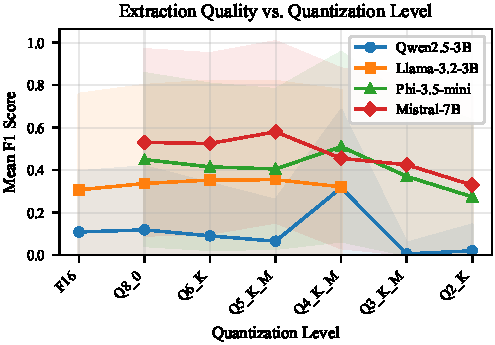
\includegraphics[width=\columnwidth]{figures/f1_vs_quant.pdf}
    \caption{Mean F1 score across quantization levels. Shaded regions show $\pm$1 standard deviation. Higher quantization (lower precision) does not uniformly degrade performance.}
    \label{fig:f1_vs_quant}
\end{figure}

Table~\ref{tab:cross_model} and Fig.~\ref{fig:f1_vs_quant} show extraction quality across quantization levels on the 100 common pages. Two key patterns emerge:

\textbf{Sweet-spot quantization.} Neither model achieves its best F1 at the highest precision (Q8\_0). Mistral-7B peaks at Q5\_K\_M (0.580 vs.\ 0.530 at Q8\_0), and Phi-3.5-mini peaks at Q4\_K\_M (0.510 vs.\ 0.449 at Q8\_0). This suggests moderate quantization may act as beneficial regularization for structured extraction tasks, or that the smaller memory footprint allows more efficient Metal GPU utilization.

\textbf{Graceful degradation at 7B scale.} Mistral-7B maintains F1$>$0.32 even at Q2\_K (2.54~GB), a 65\% size reduction from Q8\_0 (7.17~GB). Phi-3.5-mini similarly degrades gradually, with F1 dropping from 0.510 to 0.274 across the full quantization range.

For the 3B models, quantization trends are obscured by the dominant JSON validity bottleneck (Section~\ref{sec:json_validity}).

\subsection{JSON Validity as the Dominant Bottleneck}
\label{sec:json_validity}

\begin{figure}[htbp]
    \centering
    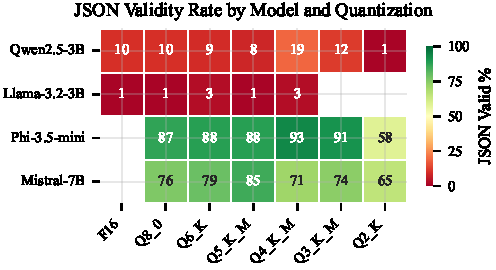
\includegraphics[width=\columnwidth]{figures/json_validity_heatmap.pdf}
    \caption{JSON validity rate (\%) by model and quantization level. The 3B models produce valid JSON in fewer than 20\% of attempts.}
    \label{fig:json_heatmap}
\end{figure}

Fig.~\ref{fig:json_heatmap} reveals a stark divide between model families. Phi-3.5-mini achieves 58--93\% JSON validity across all quantization levels, and Mistral-7B maintains 65--85\%. In contrast, Llama-3.2-3B produces valid JSON in only 1--3\% of cases, and Qwen2.5-3B in 1--19\%.

This is the primary performance bottleneck for 3B models. Their low F1 scores (0.06--0.35) reflect inability to follow the output format rather than inability to extract information. When Llama-3.2-3B does produce valid JSON, its extractions are often correct (success rate 33--39\%), suggesting the underlying extraction capability exists but is gated by instruction-following limitations.

No grammar-constrained decoding was used in these experiments, which would likely improve JSON validity for all models. This represents a clear avenue for improvement, particularly for 3B-class models.

\subsection{Inference Efficiency}

\begin{figure}[htbp]
    \centering
    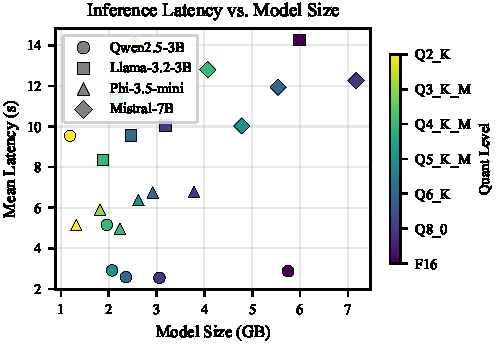
\includegraphics[width=\columnwidth]{figures/latency_vs_size.pdf}
    \caption{Mean inference latency vs.\ model file size. Marker shape indicates model family; color indicates quantization level.}
    \label{fig:latency_vs_size}
\end{figure}

Fig.~\ref{fig:latency_vs_size} shows the latency--size trade-off. Qwen2.5-3B is the fastest (2.6--5.2s per page) despite poor extraction quality. Phi-3.5-mini offers the best quality-per-second, achieving F1=0.510 at 5.0s (Q4\_K\_M, 2.23~GB). Mistral-7B requires 10--14s per page, with its optimal Q5\_K\_M variant (4.78~GB) running at 10.0s.

Quantization provides meaningful latency benefits: Mistral-7B Q5\_K\_M is 18\% faster than Q8\_0 while achieving higher F1 (0.580 vs.\ 0.530), making aggressive quantization both a quality and efficiency win.

\subsection{Input Length Effects}

\begin{figure}[htbp]
    \centering
    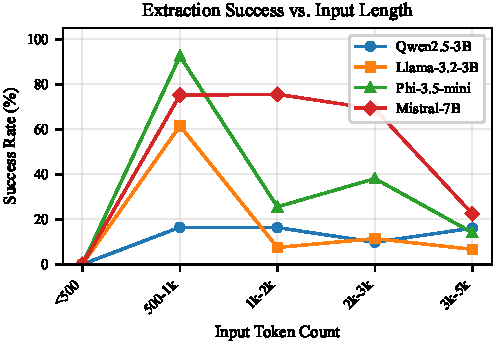
\includegraphics[width=\columnwidth]{figures/success_vs_tokens.pdf}
    \caption{Extraction success rate (F1$>$0) vs.\ input token count. All models show reduced success for very short ($<$500) and long ($>$2000) inputs.}
    \label{fig:success_vs_tokens}
\end{figure}

Fig.~\ref{fig:success_vs_tokens} shows extraction success rate as a function of input length. All models perform best in the 500--1000 token range. Very short inputs ($<$500 tokens) likely lack sufficient content for extraction. Longer inputs ($>$2000 tokens) degrade performance, especially for 3B models, suggesting context window limitations and difficulty maintaining instruction adherence with longer prompts.

Mistral-7B shows the most robust performance across input lengths, maintaining $>$70\% success rate from 500 to 3000 tokens, consistent with its larger context processing capacity.


\section{Results}
\label{sec:results}

We evaluate four small language models across multiple GGUF quantization levels on 100 web pages from the ScrapeGraphAI-100k dataset, measuring extraction quality (F1), JSON output validity, and inference latency.

\subsection{Experimental Setup}

We test four model families: Qwen2.5-3B-Instruct, Llama-3.2-3B-Instruct, Phi-3.5-mini-Instruct (3.8B), and Mistral-7B-Instruct-v0.3. Each model is quantized to up to 7 GGUF levels (F16 through Q2\_K). Mistral-7B and Phi-3.5-mini omit F16 due to memory constraints on 24GB unified RAM. Llama-3.2-3B uses Q3\_K\_L instead of Q3\_K\_M due to available model files and lacks Q2\_K; it is therefore excluded from Q3/Q2 cross-model comparisons.

All inference uses llama-cpp-python with Metal GPU acceleration, temperature 0, max\_tokens 1024, and no JSON grammar constraints. The 100 evaluation pages (37-key schemas, mean complexity 131.3) are common across all four models for fair comparison.

\subsection{Overall Performance}

\begin{table}[htbp]
\centering
\caption{Model performance summary (100 common pages, best quantization)}
\label{tab:model_summary}
\begin{tabular}{lrrrrl}
\toprule
Model & Best F1 & JSON\% & Latency(s) & Size(GB) & Best Quant \\
\midrule
Qwen2.5-3B & 0.317 & 19.0 & 5.2 & 1.96 & q4_k_m \\
Llama-3.2-3B & 0.355 & 1.0 & 11.4 & 2.16 & q5_k_m \\
Phi-3.5-mini & 0.510 & 93.0 & 5.0 & 2.23 & q4_k_m \\
Mistral-7B & 0.580 & 85.0 & 10.0 & 4.78 & q5_k_m \\
\bottomrule
\end{tabular}
\end{table}

Table~\ref{tab:model_summary} summarizes each model at its best quantization level. Mistral-7B achieves the highest F1 (0.580) at Q5\_K\_M, followed by Phi-3.5-mini (0.510) at Q4\_K\_M. Both 3B models perform substantially worse: Llama-3.2-3B reaches 0.355 and Qwen2.5-3B only 0.317.

The performance distribution is strongly bimodal. Across all configurations, only 29.4\% of extractions produce any output (F1$>$0), but among those, mean F1 is 0.77. Models either extract correctly or fail completely, with few partial results.

\subsection{Quantization Impact}

\begin{table}[htbp]
\centering
\caption{Cross-model comparison on 100 common pages (shared quantization levels)}
\label{tab:cross_model}
\begin{tabular}{llrrrr}
\toprule
Model & Quant & F1 & JSON\% & Latency(s) & Success\% \\
\midrule
Qwen2.5-3B & q8_0 & 0.118 & 10.0 & 2.5 & 15.0 \\
Qwen2.5-3B & q6_k & 0.090 & 9.0 & 2.6 & 13.0 \\
Qwen2.5-3B & q5_k_m & 0.065 & 8.0 & 2.9 & 11.0 \\
Qwen2.5-3B & q4_k_m & 0.317 & 19.0 & 5.2 & 48.0 \\
\midrule
Llama-3.2-3B & q8_0 & 0.337 & 1.0 & 10.0 & 36.0 \\
Llama-3.2-3B & q6_k & 0.353 & 3.0 & 9.6 & 38.0 \\
Llama-3.2-3B & q5_k_m & 0.355 & 1.0 & 11.4 & 39.0 \\
Llama-3.2-3B & q4_k_m & 0.321 & 3.0 & 8.3 & 35.0 \\
\midrule
Phi-3.5-mini & q8_0 & 0.449 & 87.0 & 6.8 & 62.0 \\
Phi-3.5-mini & q6_k & 0.415 & 88.0 & 6.8 & 60.0 \\
Phi-3.5-mini & q5_k_m & 0.405 & 88.0 & 6.4 & 61.0 \\
Phi-3.5-mini & q4_k_m & 0.510 & 93.0 & 5.0 & 62.0 \\
\midrule
Mistral-7B & q8_0 & 0.530 & 76.0 & 12.3 & 65.0 \\
Mistral-7B & q6_k & 0.525 & 79.0 & 11.9 & 67.0 \\
Mistral-7B & q5_k_m & 0.580 & 85.0 & 10.0 & 71.0 \\
Mistral-7B & q4_k_m & 0.455 & 71.0 & 12.8 & 60.0 \\
\bottomrule
\end{tabular}
\end{table}

\begin{figure}[htbp]
    \centering
    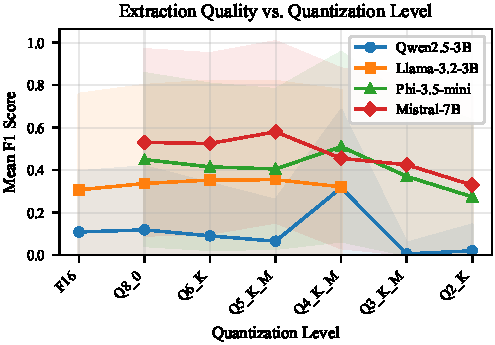
\includegraphics[width=\columnwidth]{figures/f1_vs_quant.pdf}
    \caption{Mean F1 score across quantization levels. Shaded regions show $\pm$1 standard deviation. Higher quantization (lower precision) does not uniformly degrade performance.}
    \label{fig:f1_vs_quant}
\end{figure}

Table~\ref{tab:cross_model} and Fig.~\ref{fig:f1_vs_quant} show extraction quality across quantization levels on the 100 common pages. Two key patterns emerge:

\textbf{Sweet-spot quantization.} Neither model achieves its best F1 at the highest precision (Q8\_0). Mistral-7B peaks at Q5\_K\_M (0.580 vs.\ 0.530 at Q8\_0), and Phi-3.5-mini peaks at Q4\_K\_M (0.510 vs.\ 0.449 at Q8\_0). This suggests moderate quantization may act as beneficial regularization for structured extraction tasks, or that the smaller memory footprint allows more efficient Metal GPU utilization.

\textbf{Graceful degradation at 7B scale.} Mistral-7B maintains F1$>$0.32 even at Q2\_K (2.54~GB), a 65\% size reduction from Q8\_0 (7.17~GB). Phi-3.5-mini similarly degrades gradually, with F1 dropping from 0.510 to 0.274 across the full quantization range.

For the 3B models, quantization trends are obscured by the dominant JSON validity bottleneck (Section~\ref{sec:json_validity}).

\subsection{JSON Validity as the Dominant Bottleneck}
\label{sec:json_validity}

\begin{figure}[htbp]
    \centering
    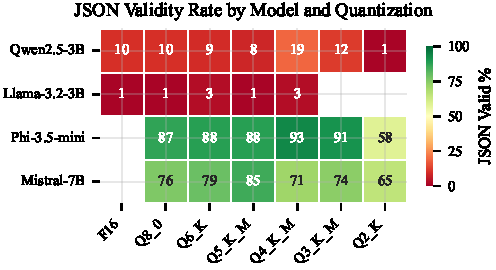
\includegraphics[width=\columnwidth]{figures/json_validity_heatmap.pdf}
    \caption{JSON validity rate (\%) by model and quantization level. The 3B models produce valid JSON in fewer than 20\% of attempts.}
    \label{fig:json_heatmap}
\end{figure}

Fig.~\ref{fig:json_heatmap} reveals a stark divide between model families. Phi-3.5-mini achieves 58--93\% JSON validity across all quantization levels, and Mistral-7B maintains 65--85\%. In contrast, Llama-3.2-3B produces valid JSON in only 1--3\% of cases, and Qwen2.5-3B in 1--19\%.

This is the primary performance bottleneck for 3B models. Their low F1 scores (0.06--0.35) reflect inability to follow the output format rather than inability to extract information. When Llama-3.2-3B does produce valid JSON, its extractions are often correct (success rate 33--39\%), suggesting the underlying extraction capability exists but is gated by instruction-following limitations.

No grammar-constrained decoding was used in these experiments, which would likely improve JSON validity for all models. This represents a clear avenue for improvement, particularly for 3B-class models.

\subsection{Inference Efficiency}

\begin{figure}[htbp]
    \centering
    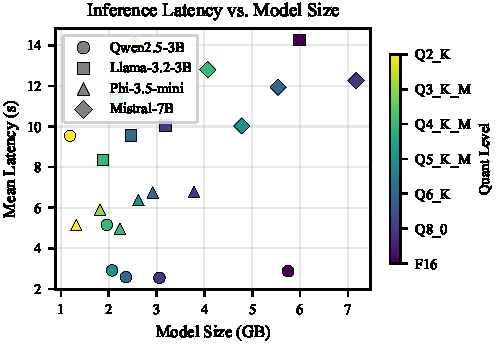
\includegraphics[width=\columnwidth]{figures/latency_vs_size.pdf}
    \caption{Mean inference latency vs.\ model file size. Marker shape indicates model family; color indicates quantization level.}
    \label{fig:latency_vs_size}
\end{figure}

Fig.~\ref{fig:latency_vs_size} shows the latency--size trade-off. Qwen2.5-3B is the fastest (2.6--5.2s per page) despite poor extraction quality. Phi-3.5-mini offers the best quality-per-second, achieving F1=0.510 at 5.0s (Q4\_K\_M, 2.23~GB). Mistral-7B requires 10--14s per page, with its optimal Q5\_K\_M variant (4.78~GB) running at 10.0s.

Quantization provides meaningful latency benefits: Mistral-7B Q5\_K\_M is 18\% faster than Q8\_0 while achieving higher F1 (0.580 vs.\ 0.530), making aggressive quantization both a quality and efficiency win.

\subsection{Input Length Effects}

\begin{figure}[htbp]
    \centering
    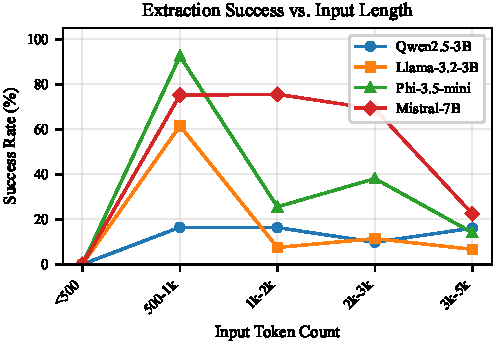
\includegraphics[width=\columnwidth]{figures/success_vs_tokens.pdf}
    \caption{Extraction success rate (F1$>$0) vs.\ input token count. All models show reduced success for very short ($<$500) and long ($>$2000) inputs.}
    \label{fig:success_vs_tokens}
\end{figure}

Fig.~\ref{fig:success_vs_tokens} shows extraction success rate as a function of input length. All models perform best in the 500--1000 token range. Very short inputs ($<$500 tokens) likely lack sufficient content for extraction. Longer inputs ($>$2000 tokens) degrade performance, especially for 3B models, suggesting context window limitations and difficulty maintaining instruction adherence with longer prompts.

Mistral-7B shows the most robust performance across input lengths, maintaining $>$70\% success rate from 500 to 3000 tokens, consistent with its larger context processing capacity.


\section{Results}
\label{sec:results}

We evaluate four small language models across multiple GGUF quantization levels on 100 web pages from the ScrapeGraphAI-100k dataset, measuring extraction quality (F1), JSON output validity, and inference latency.

\subsection{Experimental Setup}

We test four model families: Qwen2.5-3B-Instruct, Llama-3.2-3B-Instruct, Phi-3.5-mini-Instruct (3.8B), and Mistral-7B-Instruct-v0.3. Each model is quantized to up to 7 GGUF levels (F16 through Q2\_K). Mistral-7B and Phi-3.5-mini omit F16 due to memory constraints on 24GB unified RAM. Llama-3.2-3B uses Q3\_K\_L instead of Q3\_K\_M due to available model files and lacks Q2\_K; it is therefore excluded from Q3/Q2 cross-model comparisons.

All inference uses llama-cpp-python with Metal GPU acceleration, temperature 0, max\_tokens 1024, and no JSON grammar constraints. The 100 evaluation pages (37-key schemas, mean complexity 131.3) are common across all four models for fair comparison.

\subsection{Overall Performance}

\begin{table}[htbp]
\centering
\caption{Model performance summary (100 common pages, best quantization)}
\label{tab:model_summary}
\begin{tabular}{lrrrrl}
\toprule
Model & Best F1 & JSON\% & Latency(s) & Size(GB) & Best Quant \\
\midrule
Qwen2.5-3B & 0.317 & 19.0 & 5.2 & 1.96 & q4_k_m \\
Llama-3.2-3B & 0.355 & 1.0 & 11.4 & 2.16 & q5_k_m \\
Phi-3.5-mini & 0.510 & 93.0 & 5.0 & 2.23 & q4_k_m \\
Mistral-7B & 0.580 & 85.0 & 10.0 & 4.78 & q5_k_m \\
\bottomrule
\end{tabular}
\end{table}

Table~\ref{tab:model_summary} summarizes each model at its best quantization level. Mistral-7B achieves the highest F1 (0.580) at Q5\_K\_M, followed by Phi-3.5-mini (0.510) at Q4\_K\_M. Both 3B models perform substantially worse: Llama-3.2-3B reaches 0.355 and Qwen2.5-3B only 0.317.

The performance distribution is strongly bimodal. Across all configurations, only 29.4\% of extractions produce any output (F1$>$0), but among those, mean F1 is 0.77. Models either extract correctly or fail completely, with few partial results.

\subsection{Quantization Impact}

\begin{table}[htbp]
\centering
\caption{Cross-model comparison on 100 common pages (shared quantization levels)}
\label{tab:cross_model}
\begin{tabular}{llrrrr}
\toprule
Model & Quant & F1 & JSON\% & Latency(s) & Success\% \\
\midrule
Qwen2.5-3B & q8_0 & 0.118 & 10.0 & 2.5 & 15.0 \\
Qwen2.5-3B & q6_k & 0.090 & 9.0 & 2.6 & 13.0 \\
Qwen2.5-3B & q5_k_m & 0.065 & 8.0 & 2.9 & 11.0 \\
Qwen2.5-3B & q4_k_m & 0.317 & 19.0 & 5.2 & 48.0 \\
\midrule
Llama-3.2-3B & q8_0 & 0.337 & 1.0 & 10.0 & 36.0 \\
Llama-3.2-3B & q6_k & 0.353 & 3.0 & 9.6 & 38.0 \\
Llama-3.2-3B & q5_k_m & 0.355 & 1.0 & 11.4 & 39.0 \\
Llama-3.2-3B & q4_k_m & 0.321 & 3.0 & 8.3 & 35.0 \\
\midrule
Phi-3.5-mini & q8_0 & 0.449 & 87.0 & 6.8 & 62.0 \\
Phi-3.5-mini & q6_k & 0.415 & 88.0 & 6.8 & 60.0 \\
Phi-3.5-mini & q5_k_m & 0.405 & 88.0 & 6.4 & 61.0 \\
Phi-3.5-mini & q4_k_m & 0.510 & 93.0 & 5.0 & 62.0 \\
\midrule
Mistral-7B & q8_0 & 0.530 & 76.0 & 12.3 & 65.0 \\
Mistral-7B & q6_k & 0.525 & 79.0 & 11.9 & 67.0 \\
Mistral-7B & q5_k_m & 0.580 & 85.0 & 10.0 & 71.0 \\
Mistral-7B & q4_k_m & 0.455 & 71.0 & 12.8 & 60.0 \\
\bottomrule
\end{tabular}
\end{table}

\begin{figure}[htbp]
    \centering
    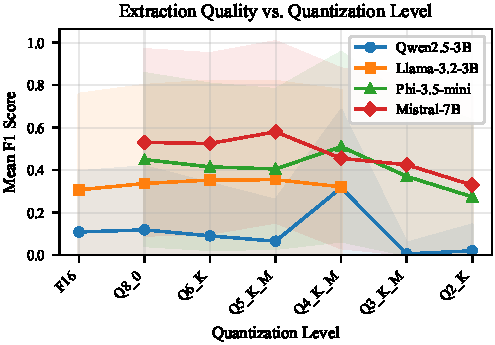
\includegraphics[width=\columnwidth]{figures/f1_vs_quant.pdf}
    \caption{Mean F1 score across quantization levels. Shaded regions show $\pm$1 standard deviation. Higher quantization (lower precision) does not uniformly degrade performance.}
    \label{fig:f1_vs_quant}
\end{figure}

Table~\ref{tab:cross_model} and Fig.~\ref{fig:f1_vs_quant} show extraction quality across quantization levels on the 100 common pages. Two key patterns emerge:

\textbf{Sweet-spot quantization.} Neither model achieves its best F1 at the highest precision (Q8\_0). Mistral-7B peaks at Q5\_K\_M (0.580 vs.\ 0.530 at Q8\_0), and Phi-3.5-mini peaks at Q4\_K\_M (0.510 vs.\ 0.449 at Q8\_0). This suggests moderate quantization may act as beneficial regularization for structured extraction tasks, or that the smaller memory footprint allows more efficient Metal GPU utilization.

\textbf{Graceful degradation at 7B scale.} Mistral-7B maintains F1$>$0.32 even at Q2\_K (2.54~GB), a 65\% size reduction from Q8\_0 (7.17~GB). Phi-3.5-mini similarly degrades gradually, with F1 dropping from 0.510 to 0.274 across the full quantization range.

For the 3B models, quantization trends are obscured by the dominant JSON validity bottleneck (Section~\ref{sec:json_validity}).

\subsection{JSON Validity as the Dominant Bottleneck}
\label{sec:json_validity}

\begin{figure}[htbp]
    \centering
    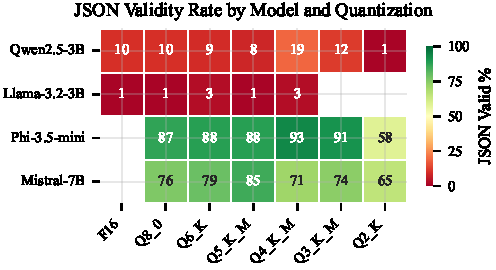
\includegraphics[width=\columnwidth]{figures/json_validity_heatmap.pdf}
    \caption{JSON validity rate (\%) by model and quantization level. The 3B models produce valid JSON in fewer than 20\% of attempts.}
    \label{fig:json_heatmap}
\end{figure}

Fig.~\ref{fig:json_heatmap} reveals a stark divide between model families. Phi-3.5-mini achieves 58--93\% JSON validity across all quantization levels, and Mistral-7B maintains 65--85\%. In contrast, Llama-3.2-3B produces valid JSON in only 1--3\% of cases, and Qwen2.5-3B in 1--19\%.

This is the primary performance bottleneck for 3B models. Their low F1 scores (0.06--0.35) reflect inability to follow the output format rather than inability to extract information. When Llama-3.2-3B does produce valid JSON, its extractions are often correct (success rate 33--39\%), suggesting the underlying extraction capability exists but is gated by instruction-following limitations.

No grammar-constrained decoding was used in these experiments, which would likely improve JSON validity for all models. This represents a clear avenue for improvement, particularly for 3B-class models.

\subsection{Inference Efficiency}

\begin{figure}[htbp]
    \centering
    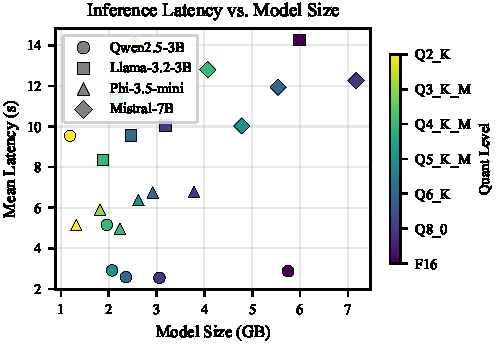
\includegraphics[width=\columnwidth]{figures/latency_vs_size.pdf}
    \caption{Mean inference latency vs.\ model file size. Marker shape indicates model family; color indicates quantization level.}
    \label{fig:latency_vs_size}
\end{figure}

Fig.~\ref{fig:latency_vs_size} shows the latency--size trade-off. Qwen2.5-3B is the fastest (2.6--5.2s per page) despite poor extraction quality. Phi-3.5-mini offers the best quality-per-second, achieving F1=0.510 at 5.0s (Q4\_K\_M, 2.23~GB). Mistral-7B requires 10--14s per page, with its optimal Q5\_K\_M variant (4.78~GB) running at 10.0s.

Quantization provides meaningful latency benefits: Mistral-7B Q5\_K\_M is 18\% faster than Q8\_0 while achieving higher F1 (0.580 vs.\ 0.530), making aggressive quantization both a quality and efficiency win.

\subsection{Input Length Effects}

\begin{figure}[htbp]
    \centering
    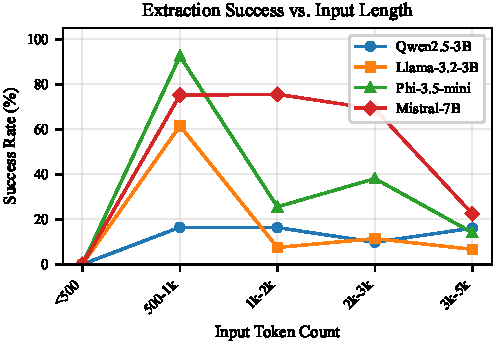
\includegraphics[width=\columnwidth]{figures/success_vs_tokens.pdf}
    \caption{Extraction success rate (F1$>$0) vs.\ input token count. All models show reduced success for very short ($<$500) and long ($>$2000) inputs.}
    \label{fig:success_vs_tokens}
\end{figure}

Fig.~\ref{fig:success_vs_tokens} shows extraction success rate as a function of input length. All models perform best in the 500--1000 token range. Very short inputs ($<$500 tokens) likely lack sufficient content for extraction. Longer inputs ($>$2000 tokens) degrade performance, especially for 3B models, suggesting context window limitations and difficulty maintaining instruction adherence with longer prompts.

Mistral-7B shows the most robust performance across input lengths, maintaining $>$70\% success rate from 500 to 3000 tokens, consistent with its larger context processing capacity.


\section{Results}
\label{sec:results}

We evaluate four small language models across multiple GGUF quantization levels on 100 web pages from the ScrapeGraphAI-100k dataset, measuring extraction quality (F1), JSON output validity, and inference latency.

\subsection{Experimental Setup}

We test four model families: Qwen2.5-3B-Instruct, Llama-3.2-3B-Instruct, Phi-3.5-mini-Instruct (3.8B), and Mistral-7B-Instruct-v0.3. Each model is quantized to up to 7 GGUF levels (F16 through Q2\_K). Mistral-7B and Phi-3.5-mini omit F16 due to memory constraints on 24GB unified RAM. Llama-3.2-3B uses Q3\_K\_L instead of Q3\_K\_M due to available model files and lacks Q2\_K; it is therefore excluded from Q3/Q2 cross-model comparisons.

All inference uses llama-cpp-python with Metal GPU acceleration, temperature 0, max\_tokens 1024, and no JSON grammar constraints. The 100 evaluation pages (37-key schemas, mean complexity 131.3) are common across all four models for fair comparison.

\subsection{Overall Performance}

\begin{table}[htbp]
\centering
\caption{Model performance summary (100 common pages, best quantization)}
\label{tab:model_summary}
\begin{tabular}{lrrrrl}
\toprule
Model & Best F1 & JSON\% & Latency(s) & Size(GB) & Best Quant \\
\midrule
Qwen2.5-3B & 0.317 & 19.0 & 5.2 & 1.96 & q4_k_m \\
Llama-3.2-3B & 0.355 & 1.0 & 11.4 & 2.16 & q5_k_m \\
Phi-3.5-mini & 0.510 & 93.0 & 5.0 & 2.23 & q4_k_m \\
Mistral-7B & 0.580 & 85.0 & 10.0 & 4.78 & q5_k_m \\
\bottomrule
\end{tabular}
\end{table}

Table~\ref{tab:model_summary} summarizes each model at its best quantization level. Mistral-7B achieves the highest F1 (0.580) at Q5\_K\_M, followed by Phi-3.5-mini (0.510) at Q4\_K\_M. Both 3B models perform substantially worse: Llama-3.2-3B reaches 0.355 and Qwen2.5-3B only 0.317.

The performance distribution is strongly bimodal. Across all configurations, only 29.4\% of extractions produce any output (F1$>$0), but among those, mean F1 is 0.77. Models either extract correctly or fail completely, with few partial results.

\subsection{Quantization Impact}

\begin{table}[htbp]
\centering
\caption{Cross-model comparison on 100 common pages (shared quantization levels)}
\label{tab:cross_model}
\begin{tabular}{llrrrr}
\toprule
Model & Quant & F1 & JSON\% & Latency(s) & Success\% \\
\midrule
Qwen2.5-3B & q8_0 & 0.118 & 10.0 & 2.5 & 15.0 \\
Qwen2.5-3B & q6_k & 0.090 & 9.0 & 2.6 & 13.0 \\
Qwen2.5-3B & q5_k_m & 0.065 & 8.0 & 2.9 & 11.0 \\
Qwen2.5-3B & q4_k_m & 0.317 & 19.0 & 5.2 & 48.0 \\
\midrule
Llama-3.2-3B & q8_0 & 0.337 & 1.0 & 10.0 & 36.0 \\
Llama-3.2-3B & q6_k & 0.353 & 3.0 & 9.6 & 38.0 \\
Llama-3.2-3B & q5_k_m & 0.355 & 1.0 & 11.4 & 39.0 \\
Llama-3.2-3B & q4_k_m & 0.321 & 3.0 & 8.3 & 35.0 \\
\midrule
Phi-3.5-mini & q8_0 & 0.449 & 87.0 & 6.8 & 62.0 \\
Phi-3.5-mini & q6_k & 0.415 & 88.0 & 6.8 & 60.0 \\
Phi-3.5-mini & q5_k_m & 0.405 & 88.0 & 6.4 & 61.0 \\
Phi-3.5-mini & q4_k_m & 0.510 & 93.0 & 5.0 & 62.0 \\
\midrule
Mistral-7B & q8_0 & 0.530 & 76.0 & 12.3 & 65.0 \\
Mistral-7B & q6_k & 0.525 & 79.0 & 11.9 & 67.0 \\
Mistral-7B & q5_k_m & 0.580 & 85.0 & 10.0 & 71.0 \\
Mistral-7B & q4_k_m & 0.455 & 71.0 & 12.8 & 60.0 \\
\bottomrule
\end{tabular}
\end{table}

\begin{figure}[htbp]
    \centering
    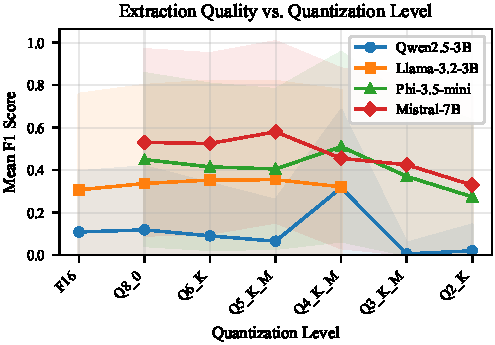
\includegraphics[width=\columnwidth]{figures/f1_vs_quant.pdf}
    \caption{Mean F1 score across quantization levels. Shaded regions show $\pm$1 standard deviation. Higher quantization (lower precision) does not uniformly degrade performance.}
    \label{fig:f1_vs_quant}
\end{figure}

Table~\ref{tab:cross_model} and Fig.~\ref{fig:f1_vs_quant} show extraction quality across quantization levels on the 100 common pages. Two key patterns emerge:

\textbf{Sweet-spot quantization.} Neither model achieves its best F1 at the highest precision (Q8\_0). Mistral-7B peaks at Q5\_K\_M (0.580 vs.\ 0.530 at Q8\_0), and Phi-3.5-mini peaks at Q4\_K\_M (0.510 vs.\ 0.449 at Q8\_0). This suggests moderate quantization may act as beneficial regularization for structured extraction tasks, or that the smaller memory footprint allows more efficient Metal GPU utilization.

\textbf{Graceful degradation at 7B scale.} Mistral-7B maintains F1$>$0.32 even at Q2\_K (2.54~GB), a 65\% size reduction from Q8\_0 (7.17~GB). Phi-3.5-mini similarly degrades gradually, with F1 dropping from 0.510 to 0.274 across the full quantization range.

For the 3B models, quantization trends are obscured by the dominant JSON validity bottleneck (Section~\ref{sec:json_validity}).

\subsection{JSON Validity as the Dominant Bottleneck}
\label{sec:json_validity}

\begin{figure}[htbp]
    \centering
    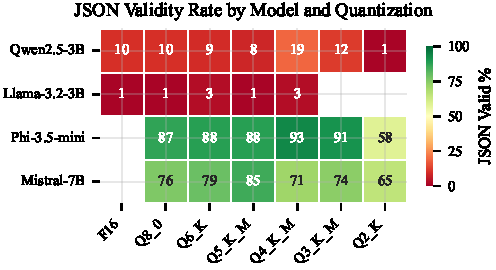
\includegraphics[width=\columnwidth]{figures/json_validity_heatmap.pdf}
    \caption{JSON validity rate (\%) by model and quantization level. The 3B models produce valid JSON in fewer than 20\% of attempts.}
    \label{fig:json_heatmap}
\end{figure}

Fig.~\ref{fig:json_heatmap} reveals a stark divide between model families. Phi-3.5-mini achieves 58--93\% JSON validity across all quantization levels, and Mistral-7B maintains 65--85\%. In contrast, Llama-3.2-3B produces valid JSON in only 1--3\% of cases, and Qwen2.5-3B in 1--19\%.

This is the primary performance bottleneck for 3B models. Their low F1 scores (0.06--0.35) reflect inability to follow the output format rather than inability to extract information. When Llama-3.2-3B does produce valid JSON, its extractions are often correct (success rate 33--39\%), suggesting the underlying extraction capability exists but is gated by instruction-following limitations.

No grammar-constrained decoding was used in these experiments, which would likely improve JSON validity for all models. This represents a clear avenue for improvement, particularly for 3B-class models.

\subsection{Inference Efficiency}

\begin{figure}[htbp]
    \centering
    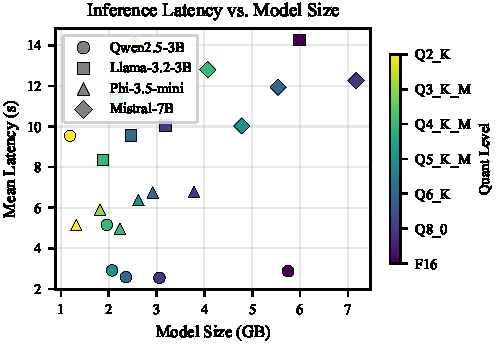
\includegraphics[width=\columnwidth]{figures/latency_vs_size.pdf}
    \caption{Mean inference latency vs.\ model file size. Marker shape indicates model family; color indicates quantization level.}
    \label{fig:latency_vs_size}
\end{figure}

Fig.~\ref{fig:latency_vs_size} shows the latency--size trade-off. Qwen2.5-3B is the fastest (2.6--5.2s per page) despite poor extraction quality. Phi-3.5-mini offers the best quality-per-second, achieving F1=0.510 at 5.0s (Q4\_K\_M, 2.23~GB). Mistral-7B requires 10--14s per page, with its optimal Q5\_K\_M variant (4.78~GB) running at 10.0s.

Quantization provides meaningful latency benefits: Mistral-7B Q5\_K\_M is 18\% faster than Q8\_0 while achieving higher F1 (0.580 vs.\ 0.530), making aggressive quantization both a quality and efficiency win.

\subsection{Input Length Effects}

\begin{figure}[htbp]
    \centering
    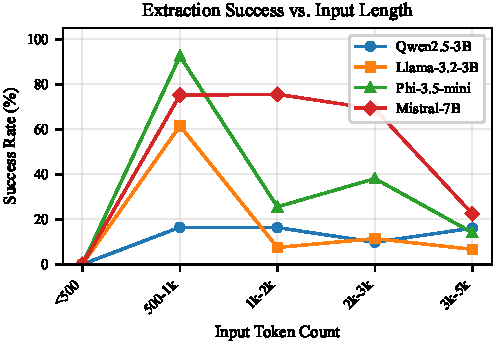
\includegraphics[width=\columnwidth]{figures/success_vs_tokens.pdf}
    \caption{Extraction success rate (F1$>$0) vs.\ input token count. All models show reduced success for very short ($<$500) and long ($>$2000) inputs.}
    \label{fig:success_vs_tokens}
\end{figure}

Fig.~\ref{fig:success_vs_tokens} shows extraction success rate as a function of input length. All models perform best in the 500--1000 token range. Very short inputs ($<$500 tokens) likely lack sufficient content for extraction. Longer inputs ($>$2000 tokens) degrade performance, especially for 3B models, suggesting context window limitations and difficulty maintaining instruction adherence with longer prompts.

Mistral-7B shows the most robust performance across input lengths, maintaining $>$70\% success rate from 500 to 3000 tokens, consistent with its larger context processing capacity.
